\documentclass[../Cours.tex]{subfiles}

\begin{document}

\setcounter{chapitre}{-1}
\chapitre{Les nombres : écriture et opérations élémentaires}

\partie{Décomposition positionnelle décimale}

\definition{Dans le système décimal usuel, il existe 10 chiffres (0;1;2;3;4;5;6;7;8;9). Les combiner permet d'écrire des nombres.}

\exemple{Avec les chiffres 1 et 2, nous pouvons écrire les nombres : 1 ; 2 ; 12 ; 21. }

\propriete{La valeur représentée par un chiffre dépend de sa position par rapport à la virgule.}

{
\small
\newcommand*\rot{\rotatebox{90}}
\begin{center}
\begin{tabularx}{\textwidth}{|*{16}{C|}}\hline
    \multicolumn{3}{|c}{Millions} & \multicolumn{3}{|c}{Milliers} & \multicolumn{3}{|c|}{Unités} & , & \multicolumn{3}{|c}{Millièmes} & \multicolumn{3}{|c|}{Millionièmes} \\\hline
    \rot{centaine de millions} & \rot{dizaine de millions} & \rot{millions} & \rot{centaine de milliers} & \rot{dizaine de milliers} & \rot{milliers} & \rot{centaines} & \rot{dizaines} & \rot{unités} & & \rot{dixièmes} & \rot{centièmes} & \rot{millièmes} & \rot{dix-millièmes} & \rot{cent-millièmes} & \rot{millionièmes}\\\hline
\end{tabularx}
\end{center}
}

\begin{listedexemples}
    \item $45,219 = (4 \times 10) + (5 \times 1) + (2 \times 0,1) + (1 \times 0,01) + (9 \times 0,001)$
    \item $\num{17845,6} = 1 \times \num{10 000} + 7 \times \num{1 000} + 8 \times 100 + 4 \times 10 + 5 \times 1 + 6 \times 0,1$
    \item $\num{2,45678} = 2 \times 1 + \frac{4}{10} + \frac{5}{100} + \frac{6}{1000} + \frac{7}{10000} + \frac{8}{100000}$
\end{listedexemples}

\clearpage
\partie{Les 4 opérations}
\souspartie{Addition}

\vocabulaire{L'addition décrit la réunion de deux quantités. Elle est notée avec le symbole $+$, les deux nombres additionnés sont les \emph{termes} et le résultat est appelé la \emph{somme}.}

\exemple{$2+3=5$ : les termes sont 2 et 3 ; la somme est 5.}

\propriete{L'addition est \emph{commutative}, c'est-à-dire que l'on obtient le même résultat en intervertissant les deux termes.}

\begin{listedexemples}
    \item $9+8=8+9$
    \item $12+17=17+12$
\end{listedexemples}

\souspartie{Soustraction}

\vocabulaire{La soustraction décrit le retranchement d'une quantité à une autre. Elle est notée avec le symbole $-$, les deux nombres sont les termes et le résultat est appelé la \emph{différence}.}

\exemple{$8-5=3$ : les termes sont 8 et 5 ; la différence est 3.}

\souspartie{Multiplication}

\definition{La multiplication est la répétition successive d'une addition. Les nombres multipliés sont les \emph{facteurs} et le résultat est appelé le \emph{produit}.}

\begin{listedexemples}
    \item << 5 fois 2 >> $ = 5 \times 2 = 2+2+2+2+2$
    \item << 3 fois 7 >> $ = 3 \times 7 = 7+7+7$ 
\end{listedexemples}

\propriete{La multiplication est \emph{commutative}, c'est-à-dire que l'on obtient le même résultat en intervertissant les deux facteurs.}

\exemples{$8 \times 7 = 7 \times 8$ ~~~~~~~~~~ $12 \times 4 = 4 \times 12$}

\souspartie{Division}

\vocabulaire{La division permet de séparer en plusieurs parts égales une quantité. On divise le \emph{dividende} par le \emph{diviseur} afin d'obtenir le \emph{quotient} et le \emph{reste}.
Les symboles utilisés pour la division sont les deux-points << : >>, le \textit{slash} << / >> et l'obélus << $\div$ >>.}

\vfill 

\begin{figure}[h!]
    \centering
    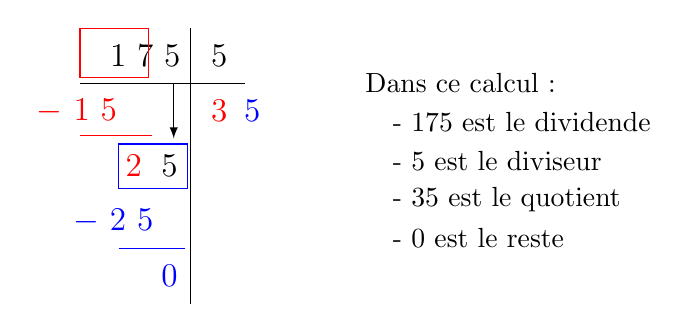
\begin{tikzpicture}[scale=0.7]
        \draw (0,0) -- (3,0);
        \draw (2,1) -- (2,-4);
        \node[anchor=east] at (2,0.5) {\large{$1~7~5$}};
        \node[anchor=west] at (2.2,0.5) {\large{$5$}};
        \draw[red] (0,0.1) rectangle (1.25,1);
        \node[red, anchor=west] at (2.2,-0.5) {\large{$3$}};
        \node[red, anchor=west] at (-0.96,-0.5) {\large{$-~1~5$}};
        \draw[red] (0,-0.95) -- (1.3,-0.95);
        \node[red, anchor=west] at (0.65,-1.5) {\large{$2$}};
        \draw[-latex] (1.7,0) -- (1.7,-1);
        \node[anchor=west] at (1.3,-1.5) {\large{$5$}};

        \draw[blue] (0.7,-1.1) rectangle (1.95,-1.9);
        \node[blue, anchor=west] at (2.8,-0.5) {\large{$5$}};
        \draw[blue] (0.7,-3) -- (1.9,-3);
        \node[blue, anchor=west] at (-0.3,-2.5) {\large{$-~2~5$}};
        \node[blue, anchor=west] at (1.3,-3.5) {\large{$0$}};

        \node[anchor=west] at (5,0) {Dans ce calcul :};
        \node[anchor=west] at (5.5,-0.7) {- $175$ est le dividende};
        \node[anchor=west] at (5.5,-1.4) {- $5$ est le diviseur};
        \node[anchor=west] at (5.5,-2.1) {- $35$ est le quotient};
        \node[anchor=west] at (5.5,-2.8) {- $0$ est le reste};
    \end{tikzpicture}
    \caption{Exemple de division posée}
\end{figure}


\end{document}